\subsection{苏斯林空间}

定义 2. 拓扑空间 X 称为苏斯林空间，如果它可度量化，且存在一个波兰空间 P 和 P 到 X 上的连续映射。拓扑空间 X 的子集 A 称为苏斯林集，如果子空间 A 是苏斯林空间。

显然每个波兰空间都是苏斯林空间，且苏斯林空间 X 在到可度量化空间 Y 中的连续映射下的像是苏斯林空间。

命题 4. 每个苏斯林空间 X 都是可数型的。

设 P 是波兰空间，f 是 P 到 X 上的连续映射。则 P 的可数稠密子集在 f 下的像是 X 的可数稠密子集。

命题 5. 苏斯林空间 X 的每个闭（相应地，开）子空间都是苏斯林的。

因为若 \(f\) 是波兰空间 \(\mathbf{P}\) 到 \(\mathbf{X}\) 上的连续映射，则在 \(f\) 之下，\(\mathbf{X}\) 的闭（相应地，开）子集的原像是 \(\mathbf{P}\) 的闭（相应地，开）子集，因而是 \(\mathbf{P}\) 的波兰子空间（第 1 号，命题 1 与命题 2）。

命题 6. 设 X 是苏斯林空间，Y 是豪斯多夫空间，\(f: \mathbf{X} \to \mathbf{Y}\) 是连续映射。则 Y 的苏斯林子空间 A 在 \(f\) 下的原像是 \(\mathbf{X}\) 的苏斯林子空间。

设 P、Q 是波兰空间，g 是 P 到 X 上的连续映射，h 是 Q 到 A 上的连续映射。设 R 是诸 \((x,y)\in\mathbf{P}\times\mathbf{Q}\) 中满足 \(f(g(x))=h(y)\) 者所成的集；R 在 \(P\times Q\) 中闭，因而是 \(P\times Q\) 的波兰子空间（第 1 号，命题 1）。设 \(\varphi\) 是投影 \(pr_{1}\) 在 R 上的限制。则 X 的子空间 \(\overline{f}^{1}(\mathbf{A})\) 是 R 在连续映射 \(g\circ\varphi\) 下的像，因而是苏斯林空间。

命题 7. 可数族苏斯林空间的积与和都是苏斯林空间。

对每个整数 n ，设 \(X_{n}\) 是可度量化空间，\(P_{n}\) 是波兰空间，\(f_{n}\) 是 \(P_{n}\) 到 \(X_{n}\) 上的连续映射。诸空间 \(P_{n}\) 的积（相应地，和）是波兰空间（第 1 号，命题 1），而此空间在诸 \(f_{n}\) 的积映射（相应地，与 \(f_{n}\) 在每个 \(P_{n}\) 上（对一切 n ）一致的映射）下的像是诸空间 \(X_{n}\) 的积（相应地，和）；后者可度量化，因而是苏斯林空间。

命题 8. 设 X 是可度量化空间，\((\mathbf{A}_{n})\) 是 X 的苏斯林子空间的序列。则诸 \(A_{n}\) 的并与交都是苏斯林空间。

这些子空间当然可度量化。诸 \(A_{n}\) 的和到 X 的子空间 \(\bigcup A_{n}\) 上的典范映射的存在性表明后者是苏斯林空间；而由第 1 号的命题 5、命题 7 与引理 1 ，\(\bigcap_{n} A_{n}\) 是苏斯林的。

\pandocbounded{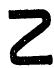
\includegraphics[keepaspectratio]{images/part002_bec1605a.jpg}}

一般说来，即使在波兰空间中，苏斯林子空间的余集也未必是苏斯林的（参看习题 6）；但参看第 6 号定理 2 的推论。

命题 9. 设 X 是可度量化空间，A 是 X 的相对紧苏斯林子空间。则存在一个紧可度量化空间 K 、K 的子集的一个递减序列 \((\mathbf{B}_{n})\) （其中每个子集都是紧集的可数并）以及一个连续映射 \(f: K \to X\) ，使得 \(A = f\left(\bigcap_{n} B_{n}\right)\) 。

必要时以 \(\overline{\mathbf{A}}\) 代替 X ，可设 X 是紧的且 A 在 X 中稠密。由于 A 是苏斯林空间，存在波兰空间 P 与连续映射 \(g: \mathrm{P} \to \mathrm{X}\) 使 \(g(\mathrm{P}) = \mathrm{A}\) 。由第 1 号定理 1 的推论 1 ，可设 P 是递减序列 \((\mathbf{U}_n)\) 的交，其中诸项是方体 \(\mathbf{I}^{\mathbf{N}}\) 的开子集。设 K 为空间 \(\mathbf{I}^{\mathbf{N}} \times \mathbf{X}\) ，它是紧且可度量化的（§ 2，第 4 号，定理 1 的推论 2）。设 \(\mathbf{G} \subset \mathbf{P} \times \mathbf{X}\) 是 \(g\) 的图像，\(\overline{\mathbf{G}}\) 是 G 在 K 中的闭包，而 \(f\) 表示 \(\mathbf{K} = \mathbf{I}^{\mathbf{N}} \times \mathbf{X}\) 到 X 上的投影；则显然有 \(f(\mathbf{G}) = \mathbf{A}\) 。由于 \(g\) 连续，G 在 \(\mathbf{P} \times \mathbf{X}\) 中闭（第 I 章，§ 8，第 1 号，命题 2 的推论 2），且 \(\mathbf{G} = \overline{\mathbf{G}} \cap (\mathbf{P} \times \mathbf{X})\) ；故 \(\mathbf{G} = \bigcap_{n=1}^{n} \mathbf{B}_n\) ，其中

\[
\mathbf {B} _ {n} = \overline {{\mathbf {G}}} \cap (\mathbf {U} _ {n} \times \mathbf {X}).
\]

由于每个 \(U_{n}\) 都是 \(I^{N}\) 中闭集的可数并（§ 2，第 5 号，命题 7），每个 \(B_{n}\) 都是紧集的可数并，证明完毕。

